% !TEX root = ../main.tex

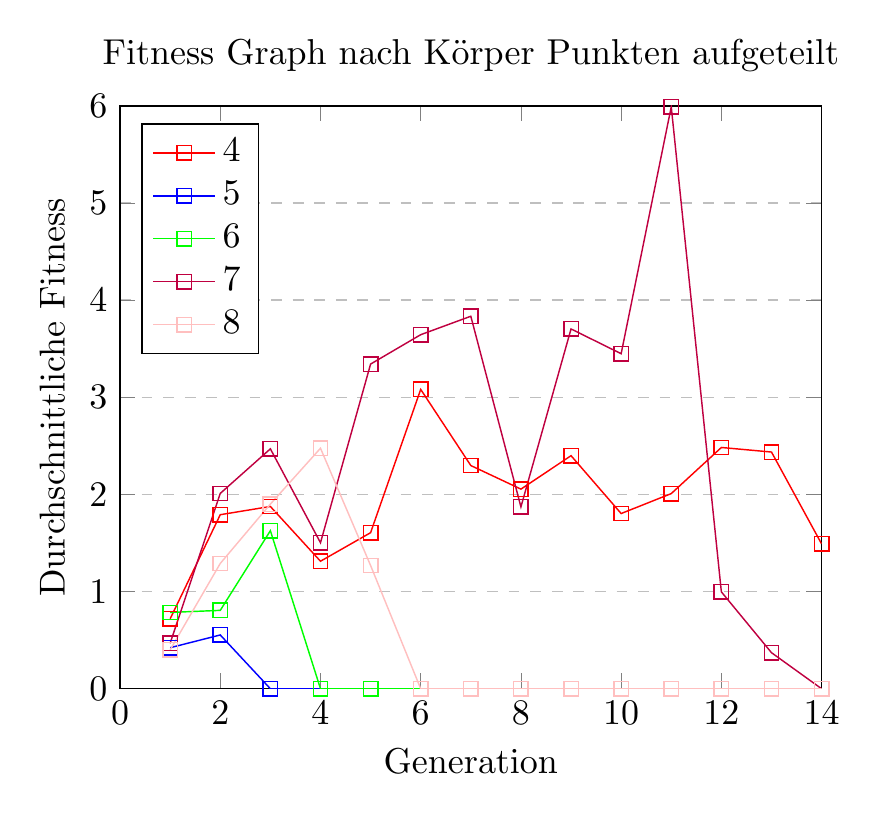
\begin{tikzpicture}[scale=1.3]
\begin{axis}[
    title={Fitness Graph nach Körper Punkten aufgeteilt},
    xlabel={Generation},
    ylabel={Durchschnittliche Fitness},
    xmin=0, xmax=14,
    ymin=0, ymax=6,
    xtick={0,2,4,6,8,10,12,14},
    ytick={0,1,2,3,4,5,6},
    legend pos=north west,
    ymajorgrids=true,
    grid style=dashed,
]

\addplot[
    color=red,
    mark=square,
    ]
    coordinates {
		(1,0.7197311288090767)(2,1.7917008390932372)(3,1.8763654203641982)(4,1.3127839017887504)(5,1.606485315324629)(6,3.081845732380266)(7,2.297797014315923)(8,2.055005581999147)(9,2.3994162926548404)(10,1.8036576432900295)(11,2.009064516425133)(12,2.4837885438165532)(13,2.436803859690654)(14,1.4910241046299537)
    };
    \addlegendentry{4}


\addplot[
    color=blue,
    mark=square,
    ]
    coordinates {
	(1,0.42241279780864716)(2,0.5535280124137276)(3,0)(4,0)(5,0)(6,0)(7,0)(8,0)(9,0)(10,0)(11,0)(12,0)(13,0)(14,0)
    };
    \addlegendentry{5}


\addplot[
    color=green,
    mark=square,
    ]
    coordinates {
	(1,0.7854441017622039)(2,0.8068950995802879)(3,1.6271000623703002)(4,0)(5,0)(6,0)(7,0)(8,0)(9,0)(10,0)(11,0)(12,0)(13,0)(14,0)
    };
    \addlegendentry{6}

\addplot[
    color=purple,
    mark=square,
    ]
    coordinates {
		(1,0.4685424281464469)(2,2.0108517235517502)(3,2.4697639744947937)(4,1.503244884001712)(5,3.3424592366328043)(6,3.644894652227138)(7,3.8348696411420136)(8,1.871792603770028)(9,3.70393052816391)(10,3.4490561534961066)(11,5.99130117893219)(12,0.9973328045823358)(13,0.37121231853961945)(14,0)
	};
    \addlegendentry{7}

\addplot[
    color=pink,
    mark=square,
    ]
    coordinates {
		(1,0.4001652509683654)(2,1.2898510225117206)(3,1.9010943668809803)(4,2.4758530855178833)(5,1.268694241841634)(6,0)(7,0)(8,0)(9,0)(10,0)(11,0)(12,0)(13,0)(14,0)
    };
    \addlegendentry{8}

\end{axis}
\end{tikzpicture}
